\documentclass{article}
\usepackage[margin=1in]{geometry}
\usepackage{amsmath}
\usepackage{listings}
\usepackage{graphicx}
\usepackage{hyperref}
\usepackage[table]{xcolor} % For coloring tables
\usepackage{array} % For custom column widths
\usepackage{calc} % For calculating widths
\usepackage{float}

\graphicspath{ {./images/} }
\setlength{\parindent}{0pt}

\title{CSP to solve Sudoku}
\author{
\begin{tabular}{rl}
    Abdullah Elsayed Ahmed & 7459\\
    Mohammad Ashraf Hamdy & 7508\\
    Samah Abdelaziz Draz & 7889
\end{tabular}    
}

\date{April 27, 2024}

\begin{document}
\maketitle
\tableofcontents

\section{Introduction}
\begin{figure}[H]
    \centering
    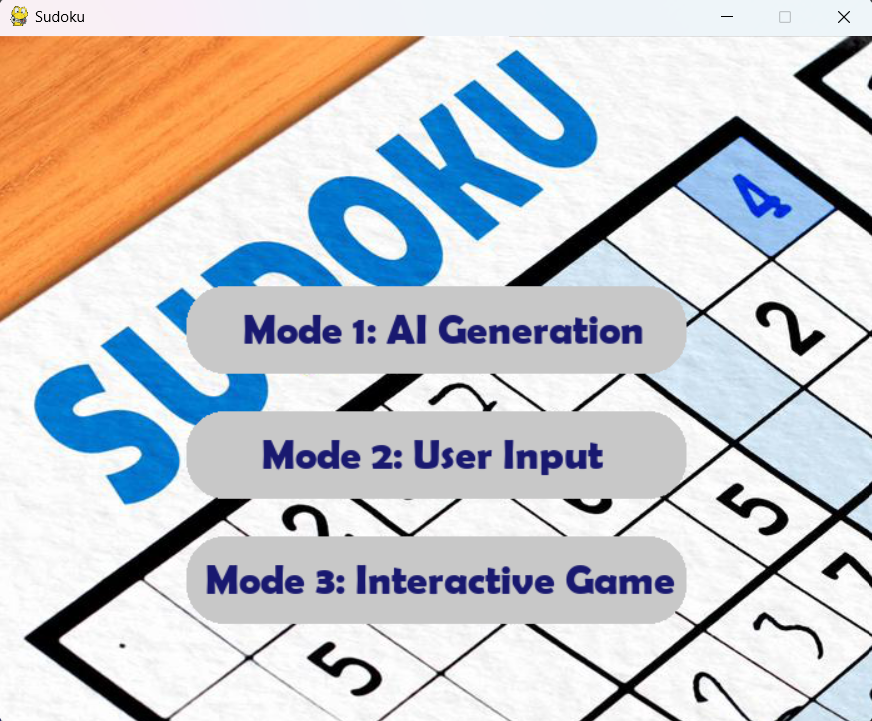
\includegraphics[width=0.7\linewidth]{GUI.png}
    \caption{Sudoku game GUI}
\end{figure}
\newpage
Sudoku can be formulated as a Constraint Satisfaction Problem (CSP) with the following components:

\begin{itemize}
  \item \textbf{Variables}: Each cell in the Sudoku grid represents a variable that needs to be assigned a value from the domain $\{1, 2, 3, 4, 5, 6, 7, 8, 9\}$. Hence, a standard Sudoku puzzle has 81 variables.
  
  \item \textbf{Domains}: The domain of each variable is restricted to the set $\{1, 2, 3, 4, 5, 6, 7, 8, 9\}$ because each cell can only hold one digit.
  
  \item \textbf{Constraints}: The constraints in Sudoku are that no two cells in the same row, column, or block can have the same value. This constraint ensures that each digit appears exactly once in each row, column, and block.
  
  \item \textbf{Solution}: A solution to the Sudoku CSP is an assignment of values to all variables (cells) such that the constraints are satisfied.
\end{itemize}

To solve Sudoku as a CSP, various algorithms can be applied, such as backtracking search with constraint propagation techniques like forward checking or maintaining arc consistency. These algorithms systematically explore the search space of possible assignments until a valid solution is found.


\section{Data structure}
\subsection*{Array}
Used to represent Sudoku board.
\subsection*{Hast table}
Used to represent the domain of each cell.
\subsection*{Domain}
Used to represent a single cell domain.
\subsection*{Queue}
Used to represent the arcs.

\section{Algorithms}
\subsection*{Backtracking}
\begin{itemize}
  \item Time complexity: $O(d^n)$
  \item Explanation: The time complexity of backtracking in the context of Sudoku solving is typically represented as $O(d^n)$, where $d$ is the depth of the search tree (the number of possibilities for each decision), and $n$ is the number of empty cells or variables that need to be filled. This exponential complexity can be mitigated by using heuristics like Minimum Remaining Values (MRV), Least Constraining Value (LCV), and constraint propagation techniques such as forward checking or maintaining arc consistency.
\end{itemize}
\newpage
\subsection*{Arc Consistency}
\begin{itemize}
  \item Time complexity (AC-3): $O(ed^3)$
  \item Explanation: Applying arc consistency to a Constraint Satisfaction Problem (CSP) involves checking and reducing the domains of variables based on constraints. The time complexity of AC-3 algorithms is $O(ed^3)$, where $e$ is the number of edges in the constraint graph and $d$ is the maximum domain size. The cubic factor arises from the need to check and update domains iteratively. 
\end{itemize}

\subsection*{LCV (Least Constraining Value)}
LCV is a variable ordering heuristic in CSPs that prioritizes assigning values to variables with the least impact on neighboring variables' domains. It helps reduce the branching factor by making informed decisions during variable assignment.

\subsection*{MRV (Minimum Remaining Values)}
MRV is a variable ordering heuristic that prioritizes variables with the fewest remaining values in their domains. It aims to handle more constrained variables early in the search, reducing the search space and potentially pruning the search tree faster.


\section{Results}
\subsection*{Easy}
\begin{center}
    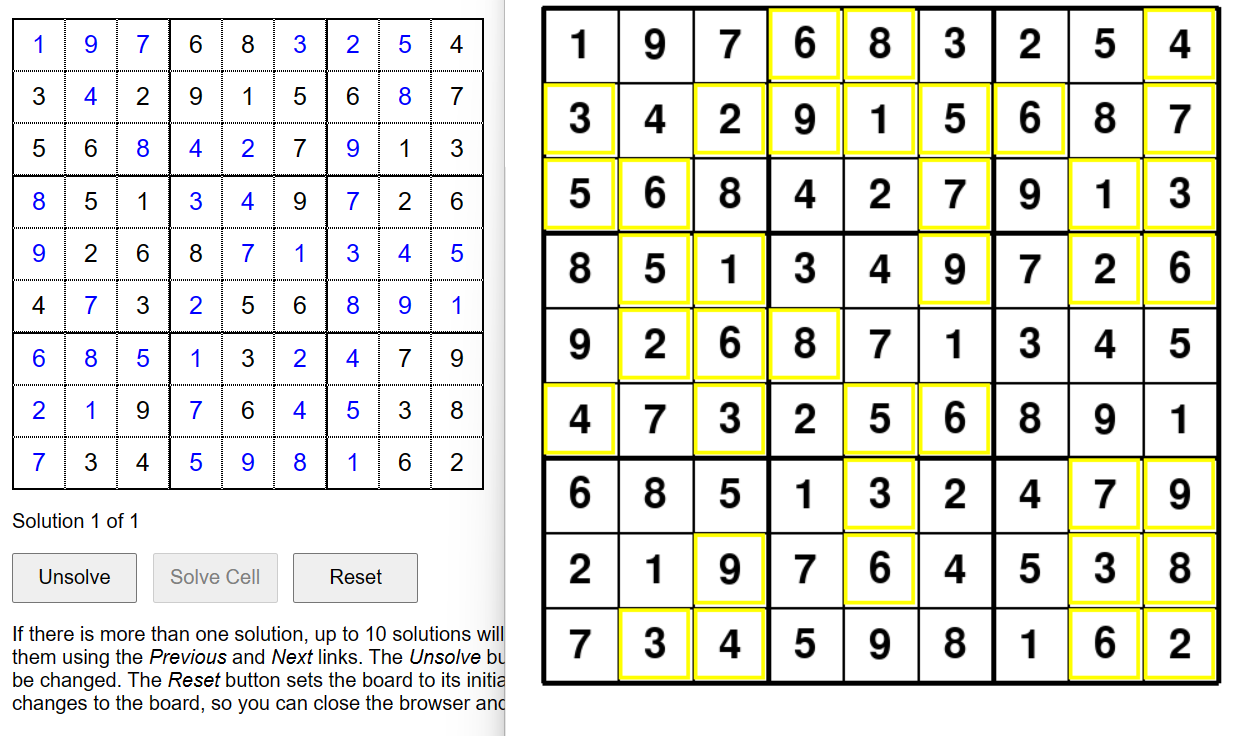
\includegraphics[width=0.8\linewidth]{easy.png}
    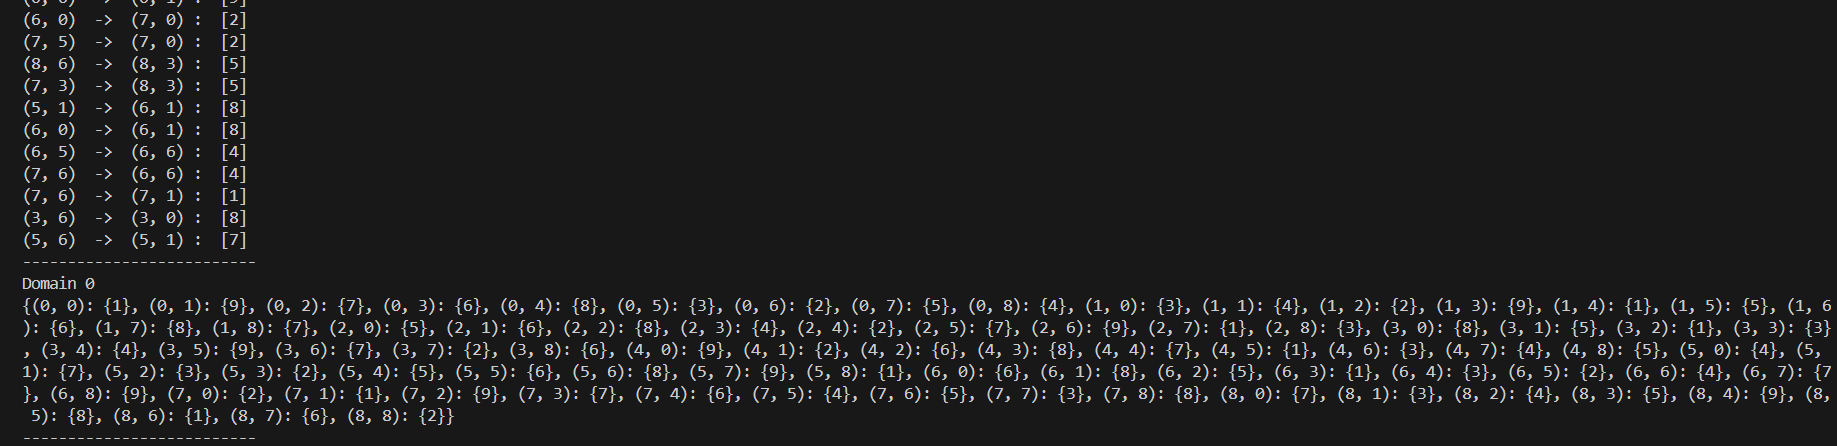
\includegraphics[width=0.8\linewidth]{easy_sample.png}
\end{center}
\begin{itemize}
    \item Time: 0.0033524036407470703
\end{itemize}
\subsection*{Medium}
\begin{center}
    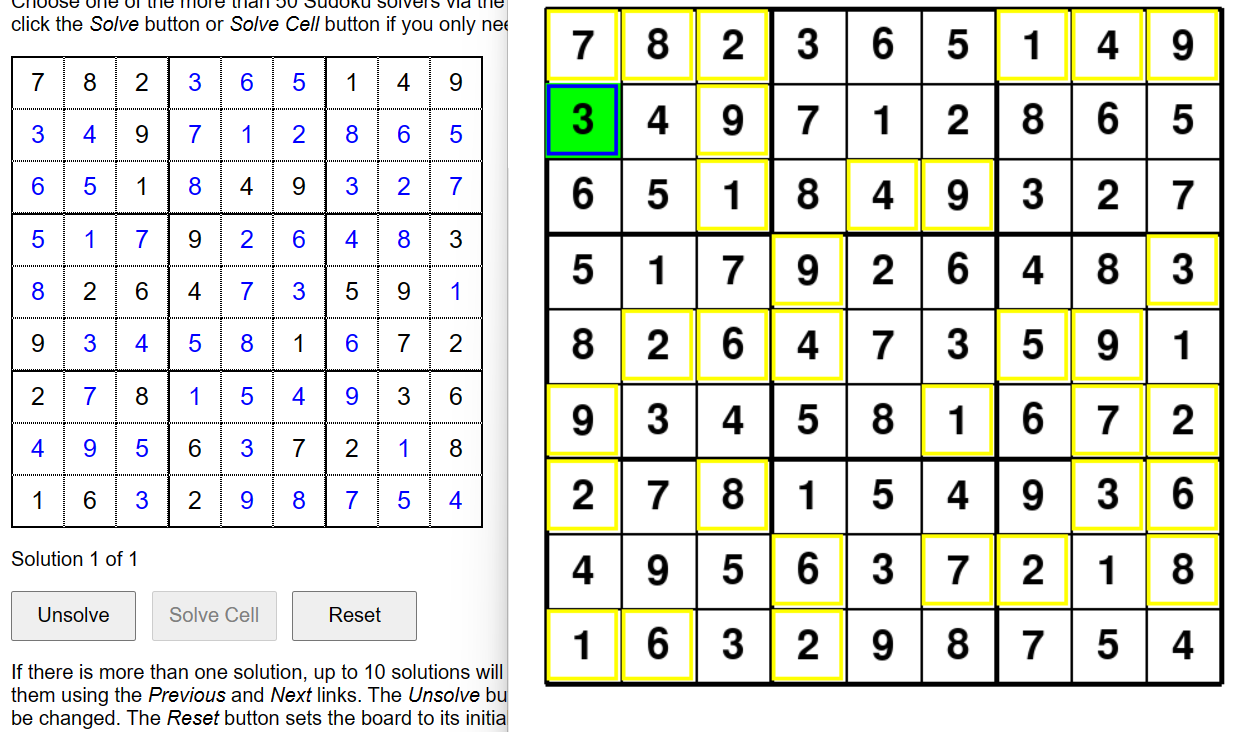
\includegraphics[width=0.8\linewidth]{Medium.png}
    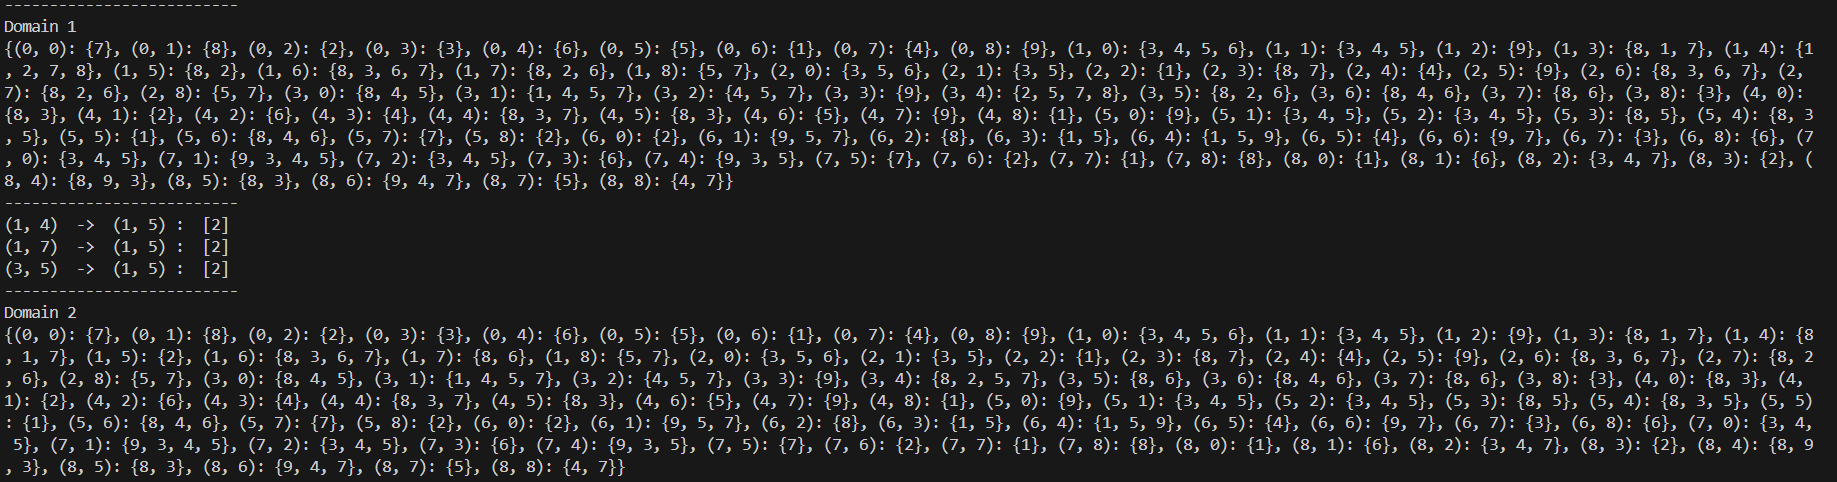
\includegraphics[width=0.8\linewidth]{Medium_sample.png}
\end{center}
\begin{itemize}
    \item Time: 0.006730318069458008
\end{itemize}
\subsection*{Hard}
\begin{center}
    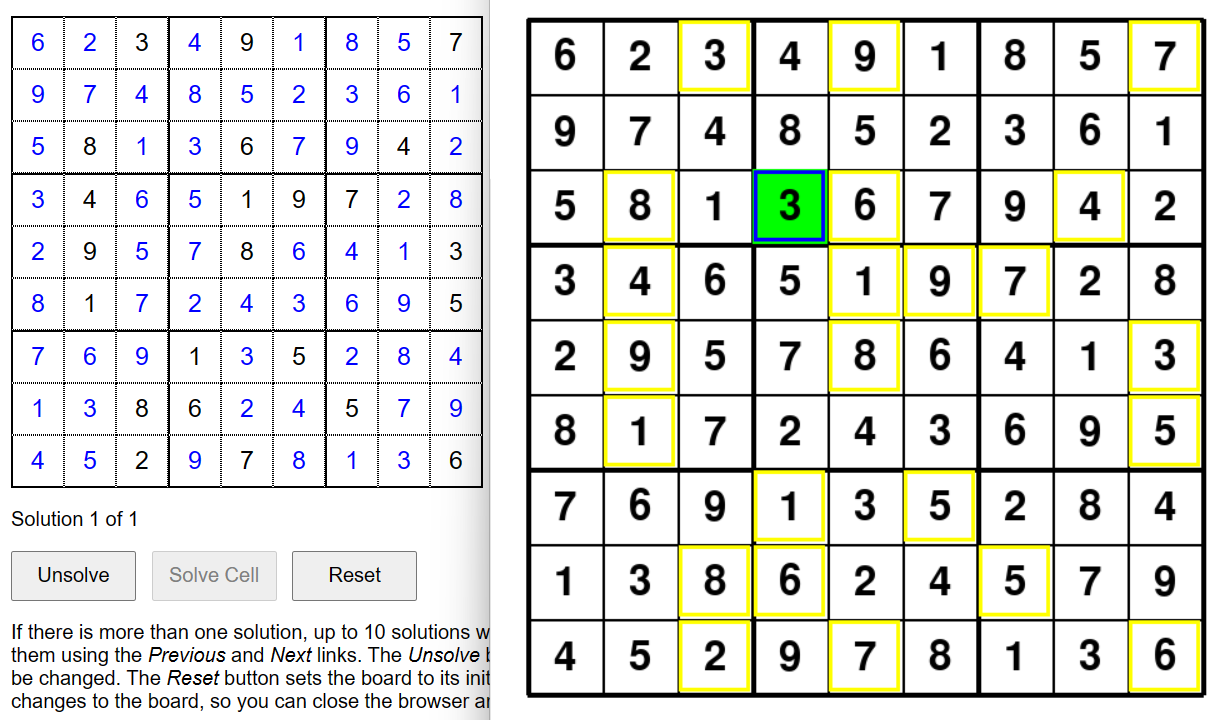
\includegraphics[width=0.8\linewidth]{VeryHard.png}
    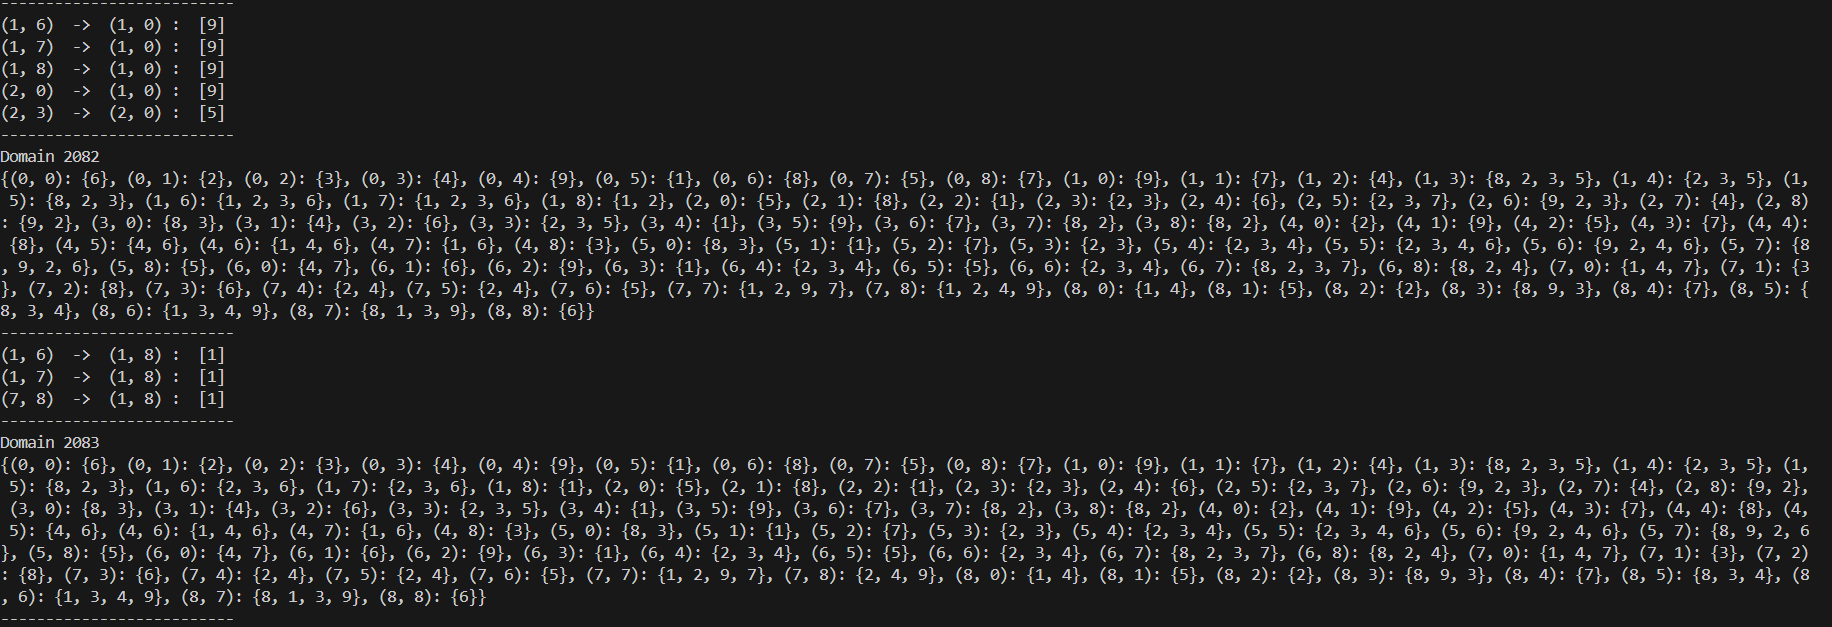
\includegraphics[width=0.8\linewidth]{VeryHard_sample.png}
\end{center}
\begin{itemize}
    \item Time: 0.0128
\end{itemize}


\end{document}